\chapter{总体设计}

激光打靶系统是一种集光、电于一体的系统,其工作原理是激光枪发出的激光束,打到光电
传感器上,经光电传感器将光信号转换为电信号,电信号经过信号处理后由单片机发送到计
算机的串行口,然后在计算机上完成成绩显示、查询和保存等功能。

激光打靶系统结构的组成框图如\cref{3-1}所示。该系统包括半导体激光枪、模块式
探测器、数字信号处理和发送电路、计算机数据处理程序等四部分。

\begin{figure}[htbp]
  \centering
  \begin{tikzpicture}
  [
    every node/.style = {font = \small, minimum height = 4.4em, minimum width = 3em}
  ]
    \linespread{1}
    \node (a) [draw, rectangle, align = center] at (0,0) {激\\光\\枪};
    \node (b) [draw, rectangle, align = center] at (2.5,0) {探测\\器\\模块};
    \node (c) [draw, rectangle, align = center] at (5,0) {滤波\\电路};
    \node (d) [draw, rectangle, align = center] at (7.5,0) {放大\\电路};
    \node (e) [draw, rectangle, align = center] at (10,0) {整形\\电路};
    \node (f) [draw, rectangle, align = center] at (12.5,0) {优先\\编码\\电路};
    \node (g) [draw, rectangle, align = center] at (2.5,-2.3) {串行\\收发\\模块};
    \node (h) [draw, rectangle, align = center] at (5,-2.3) {电平\\转换};
    \node (i) [draw, rectangle, align = center, above right] at ([yshift = -2.3cm]e.south west) {计\\算\\机};
    \draw [->, thick] (a.east) -- (b.west);
    \draw [->, thick] (b.east) -- (c.west);
    \draw [->, thick] (c.east) -- (d.west);
    \draw [->, thick] (d.east) -- (e.west);
    \draw [->, thick] (e.east) -- (f.west);
    \draw [<-, thick] (g.west) --++ (-1.5,0);
    \draw [->, thick] (g.east) -- (h.west);
    \draw [->, thick] (h.east) -- (i.west) node [midway, above = -1.5em] {串口};
  \end{tikzpicture}
  \caption{系统总体结构框图}
  \label{3-1}
\end{figure}

\section{激光的检测\cite{cn7,cn8}}

每次打靶,激光枪发出一个激光脉冲。如果激光脉冲击中光电靶,利用光生伏特效应,光电
靶上的探测器把光信号转换成电信号,因此激光的检测就是对探测器响应电信号的检测。光
电探测器的响应是一个单脉冲小信号,整个检测过程包括:信号放大、波形整形,检测输出
是标准的脉冲数字信号。

\section{靶位的划分}

把一个激光靶划分为 38 块探测器,中心 10 环为一块探测器;9.8.7.6 环分别有 8 块
探测器;5 环有 5 块探测器。根据不同靶位上的探测器来判断所击中的位置,包括环数:
10.9.8.7.6.5;偏离方向:上.下.左.右.左上.左下.右上.右下。

若信号击中两块或四块探测器的交界,则只取其中一块为有效,记为有效的探测器满足以下
条件:

\begin{enumerate}
  \item 环数高;
  \item 偏离方向为斜向(例如:上和右上两方向,选择右上)。
\end{enumerate}

根据上述要求,以及硬件电路设计的需要,对不同的探测器进行编码,见\cref{3-2}(右)。

\newpage
\begin{figure}[htbp]
  \centering
  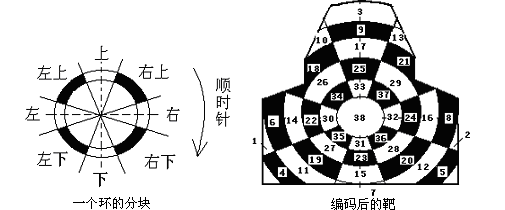
\includegraphics[width = .87\linewidth]{image-0145}
  \caption{靶位划分与编号}
  \label{3-2}
\end{figure}

\section{编码标准}

对 38 路信号按以上原则编码,编码结果如表 3-1。若脱靶无信号则记为 0 号。编码后,
每一个号码对应了每一个探测器的位置信息,包括环数和偏移方向。对信号击中两块或四块
探测器的交界的情况,只需取码号大的探测器为有效。这样,打靶的结果在硬件电路上的实现
便可由 40--6 线优先编码器完成。

\begin{table}[htbp]
  \centering
  \renewcommand{\arraystretch}{.66}
  \caption{靶位编码}
  \begin{tabular}{*{9}{@{}|@{}>{\small\centering\arraybackslash}p{.107\linewidth}}@{}|@{}}
    \hline
    & 上 & 右上 & 右 & 右下 & 下 & 左下 & 左 & 左上\\
    \hline
    10环 & \multicolumn{8}{c|}{38}\\
    \hline
    9环 & 33 & 37 & 32 & 36 & 31 & 35 & 30 & 34\\
    \hline
    8环 & 25 & 29 & 24 & 28 & 23 & 27 & 22 & 26\\
    \hline
    7环 & 17 & 21 & 16 & 20 & 15 & 19 & 14 & 18\\
    \hline
    6环 & 9 & 13 & 8 & 12 & 7 & 11 & 6 & 10\\
    \hline
    5环 & 3 & --- & 2 & 5 & --- & 4 & 1 & ---\\
    \hline
  \end{tabular}
\end{table}

\section{成绩的传送和处理}

信号经编码后发送到计算机,由计算机进行译码,在计算机上模拟显示出射击位置,对一组
结果进行统计(包括环数和方向偏移),并进行储存。

\section{其他说明}

系统分为硬件部分和软件部分。本论文主要设计制作硬件部分以及与微机的通讯的 2051 单
片机程序。微机软件部分,包括数据的处理和显示等有另外一名毕业设计同学实现。